\documentclass[12pt, a4paper]{report}

%====================== PACKAGES ======================
\usepackage[scale=0.8]{geometry}
\usepackage{tikz}
\usepackage[french]{babel}
\usepackage[utf8x]{inputenc}
\usepackage{hyperref}
\usepackage{multicol}

\newenvironment{Figure}
  {\par\medskip\noindent\minipage{\linewidth}}
  {\endminipage\par\medskip}

\usepackage{caption}

\hypersetup{
    % bookmarks=true,         % show bookmarks bar?
    unicode=false,          % non-Latin characters in Acrobat’s bookmarks
    pdftoolbar=true,        % show Acrobat’s toolbar?
    pdfmenubar=true,        % show Acrobat’s menu?
    pdffitwindow=false,     % window fit to page when opened
    pdfstartview={FitH},    % fits the width of the page to the window
    pdftitle={Rapport},    % title
    pdfauthor={Loris},     % author
    pdfsubject={Prepro},   % subject of the document
    pdfcreator={},   % creator of the document
    pdfproducer={}, % producer of the document
    pdfkeywords={}, % list of keywords
    pdfnewwindow=true,      % links in new PDF window
    colorlinks=true,       % false: boxed links; true: colored links
    linkcolor=black,          % color of internal links (change box color with linkbordercolor)
    linkbordercolor=white,
    citecolor=green,        % color of links to bibliography
    filecolor=magenta,      % color of file links
    urlcolor=cyan           % color of external links
}

\usepackage[T1]{fontenc}

\author{Loïc \textsc{Castillo} -- Loris \textsc{Croce}}

\title{\Huge\textbf{Rapport de pré-professionalisation : } \\ \emph{Enseignant-chercheur} \\ \dots\ \dots\ \dots}

\begin{document}

\maketitle{}

\tableofcontents

\chapter{Présentation du métier}

  \section{Prérequis}

    \subsection{Formation}
    Afin d'être nommé à la place d'enseignement-chercheur dans une université publique, il est nécessaire d'obtenir un doctorat. Pour l'obtenir, le cursus classique est le suite d'études universitaire LMD (Licence / Master / Doctorat). Il est parfaitement possible d'obtenir le doctorat sans suivre ce cursus, bon nombre de chercheurs ont fait une commencer par une école préparatoire, puis ont continué sur une école d'ingénieur avant de revenir sur le cheminement classique.

    \begin{Figure}
      \centering
      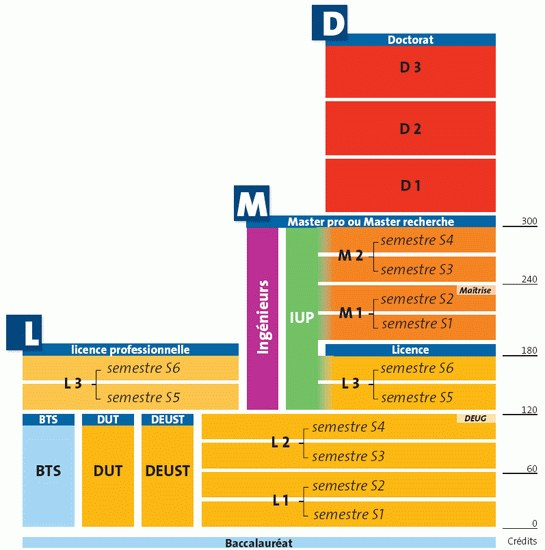
\includegraphics[width=6cm]{lmd.jpg}
      \captionof{figure}{schéma LMD}
    \end{Figure}

		% La faculté n’est donc pas le seul parcours pour devenir chercheur, en France nous avons notamment la possibilité de pratiquer le métier en entreprise après un Mas.

    \subsection{Compétences}

  \section{Types de tâches à réaliser}

    \subsection{Enseignement}

    \subsection{Recherche}

  \section{Lien avec les modules}

    \subsection{Compétences pratiques}

    \subsection{Compétences théoriques}

\chapter{Outils}

  \section{Littérature scientifique}

  \section{Autre}

\chapter{Journée des métiers}


\end{document}